%%% Document Formatting
\documentclass[12pt,fleqn]{article}
\usepackage[a4paper,
            bindingoffset=0.2in,
            left=0.75in,
            right=0.75in,
            top=0.8in,
            bottom=0.8in,
            footskip=.25in]{geometry}
\setlength\parindent{10pt} % No indent

%%% Imports
% Mathematics
\usepackage{amsmath} % Math formatting
\numberwithin{equation}{section} % Number equation per section
\DeclareMathOperator{\Tr}{Tr}
\DeclareMathOperator{\sgn}{sgn}



\newtheorem{theorem}{Theorem}
\newtheorem{definition}{Definition}
\newtheorem{hypothesis}{Hypothesis}
\newtheorem{proof}{Proof}
\newtheorem{lemma}{Lemma}
\newtheorem{example}{Example}

\usepackage{amsmath}
\usepackage{amsfonts} % Math fonts
\usepackage{amssymb} % Math symbols
\usepackage{mathtools} % Math etc.
\usepackage{slashed} % Dirac slash notation
\usepackage{cancel} % Cancels to zero
\usepackage{empheq}
\usepackage{breqn}

\newcommand{\expect}{\mathbb{E}}


% Visualization
\usepackage{graphicx} % for including images
\graphicspath{ {} } % Path to graphics folder
\usepackage{tikz}



%%% Formating
\usepackage{hyperref} % Hyperlinks
\hypersetup{
    colorlinks=true,
    linkcolor=blue,
    filecolor=magenta,      
    urlcolor=cyan,
    pdftitle={Overleaf Example},
    pdfpagemode=FullScreen,
    }
\urlstyle{same}

\usepackage{mdframed} % Framed Enviroments
\newmdenv[ 
  topline=false,
  bottomline=false,
  skipabove=\topsep,
  skipbelow=\topsep
]{sidework} %% Side-work

\usepackage{lipsum} % Lorem Ipsum example text

%%%%% ------------------ %%%%%
%%% Title
\title{Lectures Notes from Beg Rohu 2025}
\author{Clark Miyamoto (cm6627@nyu.edu)}
\date{\today}
\begin{document}

\maketitle
\begin{abstract}
	A set of lecture note from the Beg Rohu Summer School in 2025. If any of the other participants would like to collaborate on these notes, please reach out to me!
\end{abstract}

\tableofcontents
\newpage

\part{Agliari: Information Processing in Hebbian Networks}
\section{Overview}
In these lectures, we are interested in creating phase diagrams, where the macrostate is wether the neural network learns the data distribution, as we vary relevant quantities of the network (i.e. size dependence, architecture, etc.)\\
\\
We'll go over
\begin{enumerate}
	\item Intro to Hebbian Networks
	\item Hopfield Model
	\item Restricted Boltzmann Machines and Hebbian Networks
	\item Architectures
\end{enumerate}

\section{A Model for Neurons}
Our story begins with a MC Oulloch (in 1943) trying to create a mathematical model for neurons. Neurons can be effectively described as nodes on a network
\begin{itemize}
	\item Edges of the graph physical correspond to "axon" (which are paths which connect neurons).
	\item They fire electrical signals which in-turn will choose wether or not another neuron will fire.
\end{itemize}
Now let's mathematize this. A system of $\{x_i: x_i \in \{0,1\}_{i=1}^N$ neurons. They are coupled with strengths $\{J_i : J_i \in \mathbb R\}_{i=1}^N$ to an output neuron $y \in \{0,1\}$. The state equation of the system is
\begin{align}
	y = \Theta(U - U^*), ~~~ \text{s.t. }U = \sum_i J_i x_i
\end{align}
where $\Theta$ is the heaviside function, and $U^* \in \mathbb R$ is interpreted as the activation energy for the neuron to fire.\\
\\
However, neurons don't just point to one "god" neuron $y$, they all point towards each other (albeit sparsely). So our true state equation should be
\begin{align}
	x_i = \Theta (U_i - U_i^*),  ~~~ \text{s.t. }U_i =\sum_{j=1}^N J_{ij} x_j
\end{align}
Ok, this is all cool, but what if we want to generlaize our model a little more? (Specifically we'd like to recover a spin-glass system that way we can take advantage of our knowledge from statistical physics). So a couple things
\begin{itemize}
	\item Consider defining a random variable $z_i \sim \sigma_z$ where $\mathbb E[z] =0$ and $\mathbb E[z] =1$.
	\item Instead of using binary variables $\underline x = (x_1, ..., x_N) \in \{0,1\}^N$, what if we could use ising-spin variables $\underline \sigma \in (\sigma_1, ..., \sigma_N) \in \{\pm 1\}^N$. We can transform between the two using	\begin{align}
		x_i = \frac{1}{2} (1 + \sigma_i)
	\end{align}
\end{itemize}
Using this transformaiton, we can rewrite our state equation in-terms of $\underline \sigma$
\begin{align}
	\sigma_i^{(t+1)} = \text{sgn}[\varphi_k^{(t)} + T z_i^{(t)}], ~~~ \text{s.t. } \varphi_i= \sum_j J_{ij}\sigma_i^{(t)} + h
\end{align}


\begin{definition}
	The random variable $X \sim \text{Rad}(p)$ is defined to have the following properties
	\begin{align}
		\mathbb P(x=1) = 1 - \mathbb P(x = -1) = \frac{1+p}{2}
	\end{align}
\end{definition}
\begin{hypothesis}
	We assume the probability distribution over $p_Z$ is symmetric. That is $p_Z(-z) = p_Z(z)$
\end{hypothesis}
If we assume this hypothesis to hold, and define the following
\begin{align}
	g_Z(z) \equiv \int_{-\infty}^z p_Z(u) du = \mathbb P[Z < z]
\end{align}
We can show that probability of $\mathbb P [\sigma_i^{(t+1)} = \pm 1] = g_Z(\pm \frac{\varphi_i ^{(t)}}{T})$.
\\
\\
Also some notation for the future, we'll notate $p_Z(z) \equiv \frac{1}{2}[1 -\tanh^2(z)]$ and therefore $g_Z(z) =  \frac{1}{2}[1 + \tanh(z)]$.

\begin{definition}
	[Update / Dynamics] 
	We define two ways to perform dynamics
	\begin{itemize}
		\item Sequential. We select $i$ randomly, and update $\mathbb P[\sigma_i^{(t+1)}] = g(\sigma_i \varphi_i^{(t)} / T) $
		\item Parallel. $\mathbb P[\sigma^{(t+1)}] = \prod_i g(\sigma)i \varphi_i^{(t)} / T)$
	\end{itemize}
\end{definition},
Finally, we we assume the coupling matrix is symmetry $(J^T = J)$, $J_{ii} \geq 0$ and $h$ is stationary. Then the Lyaponov function
\begin{align}
	L = - \frac{1}{2} \underline \sigma^T J \underline \sigma - \underline h^T \underline\sigma
\end{align}
What's nice about this function is that is always is lowered with the dynamics we've asserted
\begin{align}
	\Delta L (\sigma, J) \leq 0
\end{align}
where $\Delta L$ is meant to be interpreted as a discrete difference in time $L(t=t'+\Delta t') - L(t=t')$. You can also show that $L$ is lower bounded.\\
\\
The result of all of this, if you run your update step, you can create a diagram which shows where you end up at fix points dependent on where you start. So if data is encoded in $\bar \sigma$, and data flows to fixed points (attractors) $\underline \xi$ depending on initialization--- we have created a classifier!
\begin{definition}
	[Attractor] We define the attractor $\xi \in \{\pm 1\}^N$, is the configuration of spins $\underline \sigma$ where you flow to a fixed point. So $\underline \xi \in \{\{ \{\pm 1\}^N\}^M$ is defines the set of attractors emitted by the model.
\end{definition}

 However, to make a \emph{good} classifier, we'd like to be able to tune/train our couplings $J$  s.t.
\begin{itemize}
	\item We can host a many attractors / stationary points
	\item The radius between the initalization and the attract is big enough s.t. we can find attractors. Aka generalize. 
\end{itemize}
\begin{definition}
	[Retrivial] A definition for when the network emits attractors
	\begin{itemize}
		\item (Strong Definition). $J = J(\xi)$ retries $\underline \xi$ staritng from $\underline \sigma$. 
		\item (Weak Definition). $\underline \xi $ is $(\delta,\epsilon)$ stable. That is when your state enter a $\delta$-radius ball away from the attractor, it will forever stay within an $\epsilon$-radius ball to the attractor.
\end{itemize}
\end{definition}
Ok, to make our life easier, assume we know what we want our attractors to be $\{\xi^\mu\}_{\mu =1}^K$, and all we need to do is tune our interaction matrix $J$. We can use \textbf{Hebb's Rule} to learn the parameters.
\begin{definition}
	[Hebb's Rule] Assert $J_{ij}  = \frac{1}{N}\sum_{\mu=1}^K \xi_i^\mu \xi_j^\mu$. The $1/N$ is to make the rule non-extensive in the number of spins $N$. We perform the update
	\begin{align}
		J^{(t+1)}_{ij} \leftarrow J_{ij}^{(t)} + \frac{1}{N} \xi_i \xi_j
	\end{align}
	We note that the time scale of the couplings $J$ is drastically different from the time scale of the neurons $\underline x$.
\end{definition}

\begin{sidework}
	In the case the number of attractors is $K=1$.
	\begin{align}
		L(\underline \sigma) & = \frac{1}{2N}\sum_{ij} \sigma_i \sigma_j \xi_i \xi_j\\
		& = - \frac{1}{2N} \sum_{ij} \tilde \sigma_i \tilde \sigma_j \geq - \frac{N}{2}
	\end{align}
	where the transformation we did was $\sigma_i \to \tilde \sigma_i \xi_i$. So we've recovered a Potts Model!
\end{sidework}
\begin{definition}
	[Motts Magnetization] We define an overlap parameter
	\begin{align}
		m_\mu \equiv \frac{1}{N} \sum_i \tilde \sigma_i = \frac{1}{N} \sum_i \sigma_i \xi^\mu_i \in [-1, +1]
	\end{align}
	What is nice about this parameter is that it allows us to access the quality of retrivial. That is if your states $\underline \sigma$ actually go to the attractor $\underline \xi$, then $m_1 \to +1$. 
\end{definition}
\begin{theorem}
	[Kohonen's Projector Rule]
	If $J$ is s.t. $\sum_j J_{ij} \xi_j^\mu = \lambda \xi_i^\mu$ for $\lambda >0$ for all $i$. Then
	\begin{align}
		\text{sgn}(J \underline \xi^\mu)=  \text{sgn}( \lambda \underline \xi^\mu) = \underline \xi^\mu
	\end{align}
	This means that $\underline \xi$ is a fixed point of the dynamics.
\end{theorem}
\subsection{Noiseless Dynamics}
Consider the following system
\begin{align}
	\xi^1 \varphi_i (\xi^1) > 0
\end{align}
If we expand this quantity this
\begin{align}
	\xi_i^1 \varphi_i(\xi^1) = \frac{\xi_i^1}{N} \sum_{j=1, j \neq i}^N \sum_\mu^K \xi_i^\mu \xi_j^\mu \xi_j^1 = \frac{N-1}{N} + \frac{1}{N} \sum_{\mu > 1} \sum_{j=1, j\neq i} \xi_i^1 \xi_i^\mu \xi_j^\mu \xi_j^1
\end{align}
We can see this leads to a signal-to-noise decomposition...


\section{Jun 9th}
Let $\underline \sigma = \{\pm 1\}^{N}$ bet a set of neurons, $\underline \xi^\mu \in \{\pm 1\}^N$ be the set of memories $\mu = 1,... , K$, and $J = \frac{1}{N} \xi \cdot \xi^T$ and $J_{ij} = \frac{1}{N} \sum_\mu \xi_i^\mu \xi_j^\mu$, with the update step
\begin{align}
	\underline\sigma^{(t+1)} = \text{sgn}(\underline \varphi^{(t)})\\
	\varphi_i^{(t)} \equiv \varphi_i(\underline \sigma^{(t)}) = \sum_j J_{ij} \sigma_j^{(t)}
\end{align}
The question we'll be answering today is $\underline \sigma = \underline \xi^\mu$ a stable solution? For simplicity let's assume $K=1$, so $\mu=1$ is our target configuraton
\begin{align}
	\xi_i^1 = \sgn(\sum_k J_{ik} \xi_k^1)
\end{align}

\begin{align}
	\xi_i^1 \sum_{j \neq i} J_{ij} \xi_{j}^1 = \underbrace{\frac{N-1}{N}}_{\mu=1, \text{ Term S}} + \frac{1}{N}\underbrace{\sum_{j \neq i} \sum_{\mu > 1, \text{ Term R}} \xi_i^1 \xi_j^1 \xi_i^\mu \xi_j^\mu}_{\mu > 1} \label{eqn:Jun9th_ExpandedTerm}
\end{align}
Note the second term is $\sqrt{(K-1)(N-1)}/N \approx \sqrt{K/N}$. So as long as $K/N \to_{N \to \infty} 0$, then the first term will be greater than the absolute value fo the second term.
\begin{sidework}
	Consider an initial configuration of the neurons $\underline \sigma^{(0)} = \underline \xi^\mu \odot \underline \chi^\mu$ where $\chi_i^\mu \sim \text{Rad}(p)$ (meaning $\mathbb P[\chi_i^\mu = \pm 1] = (1 + p)/2$) and $\odot$ is the Hammard product (element wise multiplication). This is supposed to be interpreted as a $\chi$ perturbation away from the memory $\underline \xi^\mu$.
\end{sidework}
\begin{sidework}
Consider $\underline \sigma^{(0)} = \sgn(\underline \xi^1 + \underline \xi^2 + \underline \xi^3)$. You can show it is also stable under $K/N \to 0$.\\
\\
In General $\underline \sigma^{(0)} = \sgn(\sum_{\mu=1}^L\underline\xi^\mu )$ where $L$ is odd is stable under $K/N \to 0$.
\end{sidework}
So we've seen that $K/N$ is crucial to determining stability in the system. So let's give it a name

\begin{definition} [Load] We define the \textbf{load} quantity
	\begin{align}
		\alpha \equiv \lim_{n \to \infty} \frac{K}{N}
	\end{align}When 
	\begin{itemize}
		\item $\alpha = 0$, is \textbf{low load}. 
		\item $\alpha > 0$ is \textbf{high-load}
	\end{itemize}
\end{definition}

\subsection{Hopfield Model} 
Consider the Hamiltonian
\begin{align}
	H_N(\underline \sigma; J) = - \frac{1}{N} \sum_{i < j} J_{ij} \sigma_i \sigma_j - \sum_i h_i \sigma_i\\
	\mathcal H (\underline \sigma; J) = - \frac{1}{N} \sum_{i < j} \sum_\mu \xi_i^\mu \xi_j^\mu \sigma_i \sigma_j - \sum_\mu \sum_i \xi_i^\mu h_i \sigma_i
\end{align}
where $\xi_i^\mu \sim \text{Rad(0)}$. We also introduce some notation $\omega(\dot) = \sum_{\underline \sigma} (\cdot) P_N(\underline \sigma, \underlin \xi)$, $\mathbb E[\cdot] = \sum_{\underline \xi}(\cdot)$, and $\langle \cdot \rangle _N = \mathbb E \omega_N(\cdot)$. We also denoet hte Mattis Magnetization as $m_\mu \equiv \frac{1}{N} \sum_i \xi_i^\mu \sigma_i \in [-1, +1]$.

So now going back to $\mathcal H$, we can rewrite it int this notation as
\begin{align}
	\mathcal H_N & = - \frac{1}{2N} \sum_{\mu} N m_\mu N m_\mu + \frac{1}{2} \sum_{\tau, \mu} (1) - \sum_\mu m_\mu N h_\mu\\
	& = - \frac{N}{2} \underline m^2 + \frac{K}{2} - N \underline h^T \underline m
\end{align}
Now our goal is to compute $\langle m \rangle$. We can accomplish this by computing the free energy $f_N(\xi) = \frac{1}{N\beta} \log Z_n(\xi)$ and use it as the moment generating function.































\newpage

\part{Olivier Dauchot: Swarm Robotics as Smart Active Matter}
\input{dauchot}
\newpage

\part{Julia Kempe: Synthetic Data}
Kempe's talk is titled "Synthetic Data: The Good, The Bad, The Ugly (and The Math)". I like the data.\\
\\
The premise is we are at the point where a fair amount of data on the internet has been created via AI. And we all know about model collapse (that is if you train an LLM on data generated by an ML program will eventually lead to models performing horribly). This is not so surprising because if you sample a gaussian, and fit it, then resample, on and on--- you'll find the Gaussian's variance will go down--- regression to the mean. So how can we model \& understand this phenomena!

So some causes
\begin{enumerate}
	\item Finite sample error
	\item Expressitivity error (model under capacity)
	\item Approximation error (due to optimization bias, etc.)
	\item Inteference error.
\end{enumerate}
Kempe likes to study these from the perspective of scaling laws.
\subsection{Infinite Memory Model}
This was published by Hutler in 2022.\\
\\
Consider a dataset $\mathcal D_T = \{(i_t, f(i_t))\}_{t=1}^T \subset \mathcal D$. And we have a memory model
\begin{align}
	\mathcal A(i, \mathcal D_T) = \begin{cases}
		f(i)  &  \text{if } i = \i e \text{ s.t. } \exists 1 \leq e \leq T\\
		\perp &  \text{otherwise}
	\end{cases}
\end{align}
what we notice is that $p(i) \sim i^{-\beta}$. 
There's a test error 
\begin{align}
	E_{test}(T)&  = \mathbb P(i \neq ie : i \leq \ell \leq T)) \\
	& = \sum_{i=1}^\infty p(i) (1 - p(i))^T\\
	& \simeq \sum_{i=1}^\infty i^{-\beta  } (1- i^{-\beta})^T \simeq \sum i^{-\beta e^{-(i^{-\beta})T}}
\end{align}
Let $c = 1 -1/\beta$. Then
\begin{align}
	= T^c \sum_{i} i^{-\beta} e^{-(i^{-\beta}) T}  \asymp  \Gamma(c, T k^{-\beta}) - \Gamma (c, T) = \mathcal O(1)
\end{align}
Ok... Now let's see the behavior as we retrain based off of the previous model. That is our dataset will now be $\mathcal D_T = \{(i, \mathcal A_{T_0}(i))\}_{i}$, so $\mathcal A_{T_0}(i)$ is like ChatGPT trained on very clean internet data, and this current dataset is the internet 1 year after ChatGPT.

Notice that $i$ appears $T_0 i^{-\beta}$ times in $\mathcal D_{T_0}$. So in the limit $T_0 i^{-\beta} \ll 1$. Then if $i > k$, $\mathcal A_{T_0}$ hasn't seen it.
\begin{align}
	\mathcal A'_{T_0, T}(i) = \begin{cases}
		f(i) & \text{if } i \leq k \text{ and } i=ie ~ 1 \leq \ell \leq T\\
		\perp & \text{otherwise}
	\end{cases}
\end{align}
The test error now chnage 
\begin{align}
	E_{test} = \mathbb P (i > k : 1 \leq \ell \leq T) = \sum_{i=1}^k p(i) (1-p(i))^T + \sum_{i > k}p(i) \asymp k^{-(p-1)}= k^{-c\beta}
\end{align}
If we redo this calculation in the limit $1 \ll T < k^\beta$. Then $\Gamma(c, Tk^{-\beta}) \sim \mathcal O(1)$, so 
\begin{align}
	E_{test} \asymp k^{-\beta c} + T^{-c} \asymp T^C
\end{align}

Another case $T \leq k^2$, then
\begin{align}
	E_{test} \asymp k^{-\beta c} + T^{-C} \asymp k^{-\beta c}
\end{align}
Basically, you redo this calculation over and over, and we see this scaling law apppear up everywhere. SO the test error is limited by these bounds.

\subsection{Kernel and Regression}
Consider your inputs $x \sim \mathcal N(0, \Sigma) \in \mathbb R^D$ and they're noisy $\epsilon \sim \mathcal N(0, \sigma^2) \in \mathbb R$ and the label $y = x^T W_0 + \epsilon$. Lets' start by assumping $d < T$, we have less data than parameters.
\begin{align}
	E_{test} = \mathbb E_{x, \epsilon} || x^T \hat w - y ||^2 - \sigma^2
\end{align}
The best fit $\hat w$ is via oridnary least squares between $X$ and $Y$. Meaning
\begin{align}
	\hat w & = (X_0^T  X_0)^{-1} X_0^T Y_0\\
	&  = (X_0^T X_0)^{-1} X_0^T (X_0 w_0 + E_0) & Y_0 = X_0 w_0 + E_0 \text{ (Original fit)}\\
	& = w_0 + X_0^T E_0
\end{align}
With this model, the test error we get is
\begin{align}
	E_{tot} & = ||(\hat w - w_0)||^2 \\
	& = \mathbb E_\epsilon || X_0^T E_0 ||^2\\
	& = \sigma^2 \mathbb E ~\text{Tr}(X_0(X_0^T X_0)^{-2} X_0^T )\\
	& = \sigma^2 \mathbb E ~ \text{Tr}(X_0^T X_0)^{-1}
\end{align}
Recall that $X_0 \sim \mathcal N(0, \Sigma)$, we can use some random matrix theory to compute this
\begin{align}
	& =  \sigma^2 \frac{d}{T-d-1} \sim \frac{\sigma^2 d}{T}
\end{align}
\subsubsection{Model Collapse}
So we did this just on one weight. So what happens if we do this recurisvely, over and over. Let's look at how the test error at the $i$'th iteration changes depending on the ground truth $w_0$
\begin{align}
	E_{test}^{(i)} & = || \hat w_i - w_0 ||_2\\
\end{align}
Let's start at $i=2$
\begin{align}
	E_{test}^{(2)} & = || \hat w_2 - w_0 ||_2 = || \underbrace{\hat w_2 - \hat w_1}_{X_1^T E_1}  + \underbrace{\hat w_1 - w_0}_{X_0^T E_0} ||^2\\
	& \asymp \frac{d \epsilon^2 }{T} + \frac{d \epsilon^2}{T_0}
\end{align}
Ok if we do this $n$ times
\begin{align}
	E_{test}^{(n)} = \frac{d \epsilon^2}{T} + \frac{n d \epsilon^2}{T_0}
\end{align}














\newpage

\part{Jean R\'emi King: Geometry of Thought}
\section{Overview}
Jean R\'emi King is a research at Meta Brain. In his talk he'll be going over:
\begin{enumerate}
	\item The discovery of neural codes.
	\item Evidence of convergence.
	\item Coding compositional structures.
\end{enumerate}
As an overview, the brain is obviously why humans are able to reason about the world. So the question becomes what are the \textit{exact} mechanisms which allow for reasoning? In King's research they often use an MRI and to image the brain while a participants is being shown stimuli. Experimentaly, you can show that (in a spatial sense) the brain reacting to stimuli respects locality \& hierarchy: that words go here and faces go there, and orientations of faces are within the faces section, and slightly to the side is if the face is smiling or not.\\
\\
How does machine learning come into play? Well obviously use ML to help us decode what the brain is doing (so you can perform a bayesian inference on, given brain activity, ask what is this person looking at?). If you want to see these visualizations, see Ozcelik \& van Rullen (2022), and then say wow.

\begin{definition}
	[Representation (according to King)] A representation is linearly readable information. That is if there is linear map $f$ which $\hat Y = f(X)$  approximates $Y$ quite well, then $X$ is a representation of $Y$.
\end{definition}
A very interesting application of keeping representations restricted to linear maps is attmempting to perform linear regression from brain activity to various encoders (i.e. CNN, word2vec, and ChatGPT). You can do an experiment where you map how these perform as a function of time after exposed to a word and the location in the brain, and you recover what you expect...










\newpage

\part{Yann LeCun: Self Supervised Models}
\section{Overview: A Path to Advance Machine Intelligence}
We begin with a question: why do we want to build systems that are as smart as humans? The answer is trivial lol. Obviously if they're too smart, we will live in dystopia. So the question becomes how do we construct machines with human-level intelligence? By this, he means algorithms which can generalize their knowledge to solve new problems in zeros shot. Yann believes this can be answered by \textbf{self-supervised learning.} 

He motivates his answer by noting a few things that occur in nature
\begin{itemize}
	\item Humans \& animals seem to do something quite close to self-supervised. And they are quite good at zero-shot tasks.
	\begin{itemize}
		\item I.e. look at the amount of visual data that a baby sees in it's first 4 years of life, compared to the amount of data to train a SOTA LLM. They're comparable. But the baby can do zero shot tasks, LLMS are more good at doing lookup.
	\end{itemize}
\end{enumerate}

\subsection{What is an Energy Based Model (EBM)}
Traditionally, we preform inference via a \textbf{feedforward model}. That is you run
\begin{align}
	\hat y  = (f_1 \circ f_2 \circ ... \circ f_n )(x)
\end{align}
However, you are limited by the architecture, for any inference (simple or complex) you are set to do $n$ computations. I.e. why should asking an LLM "does 2+2 =4?" use the same amount of computation as "is P=NP?". 
\\
\\
This leads us to another method, which is performing \textbf{inference via optimization}.
\begin{align}
	\hat y = \text{argmin}_{y \in \mathcal Y} f(x,y)
\end{align}
Interestingly, you can also have multiple answers as well. For training such models, you make it learn the $f_\theta$ (the \textbf{energy function}). You train this function s.t. $f$ takes low values on the training data, and it takes higher values away from the training data. Obviously we have assumed some sort of locality, that is $|\nabla f| <  \text{Constant}$-- every model makes some assumptions, it more up to you. However, because inferences require an optimization, you kinda want some notion of locality, it'll makes the optimization much easier.
\begin{sidework}
	What is the difference between energy-based models and probabilistic models? Well if you assume a Gibbs measure, and set the Hamiltonian to the energy function, you get
	\begin{align}
		p(y |x) = \frac{e^{- \beta f(x,y)}}{Z}
	\end{align}
\end{sidework}
You can also add latent parameters. Consider the energy function $E(x,y,z)$ where $z$ relates to hyper parameters of the model, etc. We can do $\min_{z\in \mathcal Z} E(x,y,z)$ are then use the resulting quantity as our new energy function.

\subsubsection{Training EBMs}
He shows how to train EBMs by walking through an Ising model example.\\
\\
A naive method is to just perform gradient descent
\begin{align}
	E(y) & = - \sum_{ij} w_{ij} y_i y_j\\
	\frac{\partial E}{\partial w_{ij}} & = - y_i y_j\\
	\therefore w_{ij} & \leftarrow w_{ij} + \epsilon (y_i y_j) & \text{Backprop Step}
\end{align}
However this is dumb, you only low energy at the specific $y$'s. You don't instill any locality. Instead do \textbf{contrastive methods}
\begin{align}
	w_{ij} \leftarrow w_{ij} + \epsilon (y_i y_j - \hat y_i \hat y_j)
\end{align}
In this case we sample $\hat y_i \in \mathcal Y$, and then move the energy function $f$ near them as well.. This allows the energy function to smoothly change. Obviously this particular method is crude, but you can implement smarter ways to do this... In summary, a contrastive method is one which not only lowers the energy function at the data point, but also lowers near by points as well...
\\
\\
The other methods are \textbf{regularized /}

\subsubsection{Avoiding Collapse in Training}




\subsection{What is a World Model}
In this quest for better intelligence, we have motivated that living creates a world model inside their head. So the next-generation of machine intelligence should also copy the same. 

Let's walk through a simple example. We can see the benefit of this approach when trying to create an agent which interacts with the world. Consider the following situation, you have an encoder $E : \text{Observations of World} \to \mathcal S_t$ a computational model of the world which takes in observations and actions $W: \mathcal S \times \text{Actions} \to \mathcal S$ and attempts to predict what the next state of the world is.  So an example of inference is
\begin{align}
	x_{t+1} = E^{-1}(W(x_t,  q)
\end{align}
where $x_t, x_{t+1} \in \mathcal S$ and $q \in \text{Actions}$. You can see this is like a optimal control problem, but we don't solve Hamilton Jacobi Equation, but instead learn the optimal result based on data.









































\newpage

\part{St\'ephane Mallat: Score Based Diffusion \& Renormalization Group Flow}
\section{Overview}
We'll be going from score-diffusion and eventually make our way to the renormalization group.\\
\\
The setup is you're given a set of input data $\{x_i : x_i \in \mathbb R^d\}_{i \leq n}$ which (we believe) to be sampled from a distribution $p(x)$. Your objective is to reconstruct this probability distribution.\\
\\
Doing this problem in the physics context, the canonical example will be attempting to recreate samples from a Ising / $\phi^4$ model. Some more advanced problems are turbulence, cosmology, metrology, and climatology. Apart from physics, you can also generate new image (i.e. conditional generation), and use it to solve inverse problems.\\
\\
As you start to think more about this problem, it might seem hopeless to learn $p(x)$. This is because the problem suffers from the \textbf{curse of dimensionality}. A crude way to calculate this is to first assume $p(x)$ is Lipschifts
\begin{definition}
	[Lipschifts] That is $| p(x) - p(x') | \leq K \underbrace{|| x- x' ||}_{\epsilon \in [0,1]^d}$
\end{definition}
This means you'll need $\sim C \epsilon^{-d}$ amount of data... You can see you're screwed.\\
\\
We can start to tackle this problem by making a key assumption, factorize the distribution
\begin{align}
	p(x) = \prod_k p_k(x) \implies \log p(x) = \sum_k \log p_k(x)
\end{align}
Two problems now emerge
\begin{enumerate}
	\item How do we choosing this factorization?
	\item How do we prevent it from just simply memorizing a distribution?
\end{enumerate} 
The first method is to assume $p(x)$ is a empirical distribution, by this I mean $p(x) = \frac{1}{n} \sum_{i=1}^n  \delta_{x_i}$ (which are get all the observed data, and draw it uniformly).

\subsection{Transport}
By \textbf{transport}, we mean constructing a new function $p_t(x)$ which is a probability distribution $\forall t$, with boundary conditions $p_{t=0}(x) =  p(x)$ and $p_{t=T}(x) = p_{gaussian}(x)$. So basically, can we find a new probability distribution which moves from complex things to NOT complex things.\\
\\
There is a \textbf{forward process}, which is some noising operator. And there is a \textbf{inverse process}, which undo's the noise (usually involves the ML algorithm). What we'll end up seeing is that these processes ends up being equivalent to RG discovered by Kadanoff \& Wilson.
\\
\\
A particular ansatz we can take is
\begin{align}
	p(x) = \underbrace{p(x_T)}_{\text{Gaussian}} \prod_{t=T+1}^1 p(x_t / x_{t-1})
\end{align}
\subsection{Outline}
\begin{enumerate}
	\item Energy Based Models, GANs, and Normalizing Flows.
	\item Score based diffusion, Fokker Planck, and denoising
	\item Generalization and memorization.
	\item Renormalization Group
	\item Particular models: simple models based on wavelet / scattering transforms.
\end{enumerate}

\section{Historical Models: Energy Based Models, GANs, Normalization Flows}
\subsection{Energy Based Models (EBM)}
When we say we have an energy based model, we have a probability distribution over $x = (x_1, ..., x_d)$ which takes the form
\begin{align}
	p_\theta(x) = \frac{e^{- U_\theta(x)}}{Z_\theta}, \ \ \text{s.t. } Z_\theta = \int dx ~e^{-U_\theta(x)}
\end{align}
\begin{example}
	An example model is a perturbation away from a Gaussian
\begin{align}
	U_\theta(x) = x^T \Sigma_\theta^{-1} x + \theta \sum_i V(x_i)
\end{align}
In physics the first one is the kinetic energy term, and the second is the potential energy term. You could start by making $U_\theta$ a neural network.
\end{example}
\begin{example}
	Another example model is the exponential family
	\begin{align}
		U_\theta(x) = \langle \theta, \Phi(x) \rangle
	\end{align}
	Notice, this is the Boltzmann distribution in physics, where $\theta \leftrightarrow \beta$ (inverse temperature) and $\Phi(x) \leftrightarrow H(x)$ (Hamiltonian)
\end{example}
\subsubsection{Likelihood}
\begin{definition}
	[Likelihood] The negative likelihood $\ell(\theta)$ of probability distribution $p$
	\begin{align}
		\ell(\theta) = - \expect_{x\sim p}{\log p_\theta(x)} = \text{KL}(p || p_\theta) + H[p]
	\end{align}
	where $\text{KL}$ is the Kullback-Lieber divergence, and $H$ is the entropy.\\
	\\
	Our objective will be choose $\theta$ s.t. we minimize the negative likelihood
	\begin{align}
		\theta^* = \text{argmin}_\theta ~ \ell(\theta)
	\end{align}
\end{definition}
To minimize this, we end up needing to calculate gradients of the likelihood. In the case of energy based models, that would mean we have to calculate the normalization $\nabla_\theta \log Z_\theta$, which in practice is quite hard. However, we can massage the problem into
\begin{align}
	\nabla_\theta \ell(\theta) & = \expect_{x \sim p} [\nabla_\theta U(x)] + \log Z_\theta\\
	& = \mathbb E_{x \sim p}[\nabla_\theta U_\theta(x)]- \expect_{x \sim p_\theta}[\nabla_\theta U_\theta(x)]
\end{align}
So now the problem becomes figuring out how to compute $\expect_{x \sim p_\theta}$ which involves spending time to construct a Markov Chain Monte Carlo method.

\subsection{GANs}
GAN stands for Generative Adversarial Network, the original paper is by Goodfellow \& Bengio (2014). What you do is you construct two neural networks $G_{\theta_G}$ and $D_{\theta_D}$ and make their tasks adversarial to one another. $G$'s task is to generate images from noise $z \sim \mathcal N(0,1)$, and $D$'s task is to figure out which image was real vs generated. So to recap, $G: z \to \text{Images}$ and $D: \text{Images} \to [0,1]$, where your goal is that 
\begin{align}
	D(x) & = \begin{cases}
		1 & \text{if } x \text{ is a real image}\\
		0 & \text{if } x \text{ is a fake image}
	\end{cases}
\end{align}
The loss function is
\begin{align}
	\mathcal L(\theta_D, \theta_G) & = \mathbb E_{x \sim p_{data}}[\log D(x)] + \mathbb E_{z \sim \text{Gaussian}}[\log (1 - D(G(z))]\\
	\text{where } D(x) & = \begin{cases}
		1 & \text{if } x \text{ is a real image}\\
		0 & \text{if } x \text{ is a fake image}
	\end{cases}
\end{align}
What ends up happening in practice is that GANs almost always memorize the data instead of learning to gneerate. Another way of saying this is this is a difficult nash-equilibrium to obtain, or you see \textbf{mode collapse}. This is why people used them for image generation, and couldn't use them for physics data...\\
\\
A small aside... If you successfully find the global minimizer/maximizer
\begin{lemma}
	The optimal discriminator ends up being
	\begin{align}
		D^* & = \text{argmax}_D ~\mathcal L(D,G)\\
		& = \frac{p_{data}(x)}{p_{data}(x) + p_{G}(x)}
	\end{align}	
\end{lemma}
\begin{theorem}
	\begin{align}
		\min_G \max_D \mathcal L(D,G) \iff p_G = p_{data}
	\end{align}
\end{theorem}
Both are theoretical results, so they don't consider using finite number of samples.

\subsubsection{Conditional GANs} What if you want to condition your learned distribution on some variables (i.e. text to image, or in-painting). Your loss function will be
\begin{align}
	\mathcal L(D,G) = \mathbb E_{p_{data}} [\log D(x | y)] + \mathbb E_{z \sim p_{data}} [\log (1 - D(G(x|y)))]
\end{align}

\subsection{Normalizing Flows}
In this problem, we have an easy to sample distribution $p_z$ (which is Gaussian), and difficult to sample distribution $p_x$ (which is the target distribution). The way we'll do transport is to learn a diffeomorphism $T_\theta$, and now we can do change of basis between the two
\begin{align}
	p_x(x) = p_z(T(x)) \det \mathcal J_{T}(x) 
\end{align}
where $\mathcal J_{T}$ is the Jacobian of $T$.

The likelihood ends up being
\begin{align}
	\ell(\theta) = - \mathbb E_{x \sim p} [\log p_z(T_\theta(x))] - \mathbb E_{x \sim p}[\log |\det - \mathcal J_{T_\theta}| ]
\end{align}
You may be thinking that the normalization constant (2nd term) looks quite scary... However with the right ansatz, it's analytically tractable. Here's how to do it.

First, break the diffeomorphism into smaller diffeomorophisms $T^{-1}_\theta = T_1^{-1} ... T_k^{-1}$. So the infal term becomes $\log |\det \mathcal J_{T_\theta}(x)| = \sum_i \log |\det \mathcal J_{T_i}(x_i)|$. 

Second, we can use block inverse formula to get a nice closed form expression. To keep track of the block inverse, let's split up $x \in \mathbb R^d = (x_0, x_1) \in \mathbb R^{d_0} \times \mathbb R^{d_1}$ 
\begin{align}
	T_\theta(x) & = (x_0, e^{S_\theta(x_0)} \odot x_1 + t_\theta(x_0))\\
	T_\theta^{-1}(z) & = (z_0, (z_1 - t_\theta(z_0)) \odot e^{-S_\theta (z_0)}
\end{align}
where $\odot$ denotes the Hadamar product, and $z = (z_0,z_1)$. You can now show that the $\log \det$ term picks up a nice expression
\begin{align}
	\implies \log |\det \mathcal{J}_{T_\theta}(x)| = \sum_{i=1}^d s_\theta(x_0)
\end{align}
Finally we have our likelihood
\begin{align}
	\ell(\theta) = - \mathbb E_{x \sim p} [\log p_z(T_\theta(x))] - \sum_{i=1}^d \mathbb E_{x \sim p}[ s_\theta(x_0)]
\end{align}

\subsubsection{Continuous Flow}
Consider the \textbf{Neural ODE}
\begin{align}
	\frac{dx_t}{dt} & = v_\theta(x_t,t) & \text{(Continuous)}\\
	x_{t+\epsilon} & = x_t + \epsilon~ v_\theta(x_t, t) & \text{(Naive Discretization)}
\end{align}
where $v_\theta : \mathbb R^d \times [0,1] \to \mathbb R^d$ is a residual (skipped connections) neural network, which is assumed to be Lipshifts.\\
\\
However, what if we want to stop thinking about transporting just particles, but rather transporting probability distribution mass? Recall the \textbf{Liouville Equation}
\begin{align}
	\frac{\partial p_t}{\partial t} & = - \nabla \cdot (v_t ~p_t)\\
	& = - \underbrace{v_t \cdot \nabla p_t}_{\text{Convection}} - \underbrace{p_t (\nabla \cdot  v_t )}_{\text{compression / dilation}}
\end{align}
Why would you want to do this? In metrology, it's quite difficult to make a point estimate of the future (due to chaoticity of fluid dynamics), so instead what if we make a probabilistic inference! This frame work more well posed! 

\subsection{Score Based Diffusion}
If you want to add diffusion, you recover the \textbf{Fokker Planck Equation}
\begin{align}
	\frac{\partial p_t}{\partial t} = - \nabla \cdot (p_t(x) v_t) - \Delta \left(\frac{1}{2} \sigma^2(x) p_t(x) \right)\iff dx_t = v_t(x_t) dt + \sigma dW_t \label{eqn:FokkerPlanck}
\end{align}
where $\Delta$ is the Laplacian operator, where we interpret $\text{Law}(x_t) = p_t$. 

\begin{sidework}
	These ideas were developed by Physicists Reckstein \& Ganguli at Stanford in 2015. It took a whole 5 years within the same university to make its way to the CS department where Song \& Enman published their seminal paper. 
	\\
	\\
	However this has been thought about from a signal processing perspective by Zhadoki \& Semaicelli, and Horr \& et al.
\end{sidework}
Now we can finally begin Score Based Diffusion!
\subsubsection{Orstein Ulhrbeck SDE}
Consider the stochastic differential equation
\begin{align}
	dx_t = - \kappa x_t dt + \sigma dW_t
\end{align}
To solve it, perform the change of variable 
\begin{align}
	y_t &= e^{\kappa t} x_t\\
	dy_t &= e^{\kappa t} (- \kappa x_t  dt + \sigma dW_t) + \kappa  e^{\kappa t}x_t dt = e^{\kappa t} \sigma dW_t
\end{align}
This yields 
\begin{align}
	x_t = e^{-\kappa t} x_0 + \sigma \sqrt{\frac{1 - e^{-2 \kappa t}}{2 \kappa}} z
\end{align}
where $z \sim N(0,\mathbb I)$. Inspecting the limiting cases of our solution, $x_{t=0} = x_0$ and $x_{t \to +\infty} = \frac{\sigma}{2\sqrt{2\kappa}} z$. So this is a process is a linear interpolation between our input $x_0$ and white noise $z$. 
\begin{sidework}
	Consider the $\kappa=1$ Orstein Ulhbreck SDE.
	\\
	\\
	Moving to the distribution picture, we can see
	\begin{align}
		p_t = (e^{\kappa t} p(\cdot e^{\kappa t})) * g_\sigma
	\end{align}
	where $g_\sigma = \mathcal N(0, 1-e^{-2 \kappa t})$. We can also see this forms a semi-group, we don't get an inverse for free...
	\\
	\\
	Another way to see this is to Fourier transform. Generically if you have $h = f * g$, then $\hat h = \hat f \hat g$. In our case $\hat g(\omega) \sim e^{- (1-e^{-2 \kappa t}) ||\omega||^2/2}$. You can see this expression explodes as time goes on
\end{sidework}
\subsubsection{Denoising}
Now our task is to denoise the OU process. For notation, let's use $y_t = x_{T-t}$ and $q_t = p_{T-t}$.  We can plug our $q_t$ into the Fokker Planck (\ref{eqn:FokkerPlanck}), and derive a time evolution on the distribution for the reverse process
\begin{align}
	\frac{\partial p_t}{\partial t} + \nabla \cdot (- p_t x_t) - \Delta p_t & = 0 & \text{Forward in time}\\
	\implies  \frac{\partial q_t}{\partial t} + \nabla \cdot (q _t y_t) + \Delta q_t & = 0 & \text{Backwards in time}
\end{align}
Notice your have inverse diffusion, which is completely unstable. Show how can we rewrite this to become more stable? Notice the trick
\begin{align}
	\Delta q_t = \nabla \cdot (q_t \underbrace{\nabla \log q_t}_{\text{score}})
\end{align}
We finally get
\begin{align}
	\frac{\partial q_t}{\partial t} + \nabla \cdot (q_t y_t - (1+\alpha) q_t \nabla\log p_t) - \alpha \Delta q_t = 0\\
	dy_t = [y_t + (1+\alpha) \nabla \log q_t] + \sqrt{2\alpha}~ dW_t
\end{align}
We now have a generic way to talk about the reverse-time process!

\subsubsection{Denoising OU}
We have the $\kappa=1$ OU, 
\begin{align}
	x_t = e^{-t} x + \sqrt{1 - e^{-2 t}} z
\end{align}
Taking the coordinate change $\tilde x_t = e^{t x_t}$, you now find at each point in time, you observe $y_t$
\begin{align}
	y_t = x + \sqrt{e^{2t} - 1}z
\end{align}
Recall we are attempting to denoise this process. In signal processing, your trying to minimize the mean square error 
\begin{align}
	\mathbb E_{x,z} [||\hat x(y_t) - x||^2]
\end{align}
So given an observed noisy input $y_t$, can we construct a $\hat x$ (which takes in $y_t$) and yields $x$. We can use \textbf{Tweety's Formula} to construct the optimal denoiser
\begin{theorem}
	The optimal denoising of the OU process is
	\begin{align}
		\hat x (x_\sigma) = x_\sigma + \sigma^2 \nabla_{x_\sigma} \log p_\sigma (x_\sigma)
	\end{align}
	Proof:
	\begin{align}
		p_\sigma (x_\sigma) & = \int p(x_\sigma | x) p(x) dx\\
		\nabla p_\sigma (x_\sigma) & = \int g_\sigma (x_\sigma - x) p(x) dx & \text{Due to solution of OU}\\
		& = \frac{1}{\sigma^2} \int  (x_\sigma - x) g_\sigma(x_\sigma - x) p(x) dx\\
		\frac{\sigma^2 \nabla p_\sigma(x_\sigma)}{p_\sigma(x_\sigma)} &  = \int (-x_\sigma + x) p_\sigma(x | x_\sigma) dx & p(x) / p_\sigma(x_\sigma) = p_\sigma(x | x_\sigma)\\
		& = - x_\sigma + \hat x(x_\sigma) 
	\end{align}
	where $g_\sigma(x_\sigma -x ) = C_\sigma e^{-||x_\sigma - x||^2 / 2\sigma^2}$ is a Gaussian distribution. You can now see where the fomrula comes from!
\end{theorem}
Plugging in Tweedy's Formula into the mean square error
\begin{align}
	\mathbb E_{x,z} [|| ]
\end{align}
As a machine learning person, once you see, "minimize square error", you should just plug that into a neural network and let it rip. So your loss function becomes
\begin{align}
	\mathcal L(\theta) =  \Big|\Big|\frac{\hat x_\theat(x_\sigma) - x}{\sigma^2}\Big|\Big|^2
\end{align}




























\newpage
hi



\newpage

\part{Marc M\'ezard: Statistical Physics of Generative Diffusion}
\section{Overview}
\begin{enumerate}
	\item Langevin-Fokker Planck \& Ornstien Uhlenbeck
	\item Principles of Generative Diffusion
	\item A simple case: Gaussian Data
	\item Aside: Related approaches ODE and Stochastic Localization \& Interpolants
	\item Intermission: Thermodynamic Score
	\item A harder case: Curie Weiss
	\item Speciation Transition: Classifier Free Guidance
	\item Generalization vs Memorization
\end{enumerate}

\section{Recall: Stochastic Processes}
\subsection{Langevin Equation}
Let $x \in \mathbb R^d$, and has the state equation
\begin{align}
	\frac{dx}{dt} = F(x) + \eta(t)
\end{align}
where $F: \mathbb R^d \to \mathbb R^d$ is the force field, and $\eta(t)$ is a Gaussian with properties $\langle \eta(t)\rangle = 0$ and $\langle \eta(t) \eta(t') \rangle = 2 \delta(t - t')$. In stochastic process notation it is
\begin{align}
	dx_t = f(x) dt + \sqrt{2	} dW_t
\end{align}
\begin{sidework}
	In general, Mezard will work in continuous time. However whenever we want to make a comment about implementations on a computer, we'll use the Ito descretization.
	\begin{align}
		x(t + \delta t) = x(t) + \delta t ~F(x(t)) + \int_{t}^{t + \delta t} d\tau \eta~ (\tau)
	\end{align}
	and
	\begin{align}
		\delta x = \delta t F(x(t)) + \sqrt{2 \delta t} z_t
	\end{align}
	where $z_t$ is a unit gaussian.
\end{sidework}
\begin{sidework}
	Note the integral of the time-dependent gaussian is given by
	\begin{align}
		\langle y \rangle := \int_t^{t+\delta t} \eta (\tau) d \tau
	\end{align}
	has the following properties $\langle y \rangle = 0$ and $\langle y^2\rangle = 2 \delta t$.
\end{sidework}
\subsection{Fokker Planck}
Consider the conditional distribution $p_t(x | x_0)$, the equation which keeps it probabliity distribution is the Fokker Planck equation
\begin{align}
	\frac{\partial p_t}{\partial t} = \Delta p_t - \nabla \cdot  (F p_t)
\end{align} 
where $F$ is a vector field. You can then ask what's condition of the stationary distribution, that is $\partial_t p_t = 0$, it must satisify
\begin{align}
	\Delta p_t + \nabla \cdot (p \nabla V) = 0\\
	p_{stationary}(x') = \frac{1}{Z} e^{-V(x)}
\end{align}
Note that our usage of $\sqrt{2}$ in the previous section was to ensure we get a temperature $\beta = 1$.

\subsection{Ornstein Uhlenbeck}
This is when $V(x) = \frac{1}{2} |x|^2$. So the Langevin equation becomes
\begin{align}
	\dot x = F(x) + \eta(t) \implies \dot x = - x + \eta(t)
\end{align}
and your stationary distribution becomes
\begin{align}
	p_{st}(x) = e^{-|x|^2 / 2}
\end{align}
\begin{sidework}
	For example, if you have $x(t=0) = a \in \mathbb R^d$. Then the solution to the Langevin becomes
	\begin{align}
		x(t) = a e^{-t} + \int_0^t e^{-(t-\tau)}\eta(\tau) d\tau
	\end{align}
	the second term is equivalent to the random variable $\mathcal N(0, 1-e^{-2t})$, and we'll notate $\Delta t = 1-e^{-2t}$.
\end{sidework}
So you can interpret this process as something which always goes to white noise.
\subsection{General Time and Variance}
Consider the equation
\begin{align}
	\frac{dx}{dt} = f(t) x(t) + g(t) \eta(t)
\end{align}
previously $g = 1$, but now $f: \mathbb R^d \to \mathbb R^d$ and $g: \mathbb R^d \to \mathbb R^d$. Solving the equation with the same boundary condtion as before ($x(t=0) = a)$, you get
\begin{align}
	x(t) & = a s(t) + s(t) \sigma(t) z(t)\\
	& \text{s.t. }\begin{cases}
		s(t) = \exp\left[ \int_0^t d\tau ~f(\tau) \right]\\
		\sigma(t)^2 = 2 \int_0^t d\tau \left (\frac{g(\tau)}{s(\tau)} \right)^2
	\end{cases}
\end{align}
\begin{sidework}
	Example: Brownian Motion is recovered when $f=0$ and $g = 1$.
\end{sidework}

\section{Principals of Generative Diffusion}
\begin{sidework}
	For some background reading for this section there's: Sohl-Dickstein et al (2015), Yang Song \& Stefano Ermon (2019), and a Review by Ling Yang et al (ArXiv:2209.00796). 
\end{sidework}
In generative modeling, \emph{the problem setup} is that you have an a target distribution $p_0(a)$ s.t. $a\in \mathbb R^d$, however you only have an empirical estimation of said target distribution $\{a^\mu\}_{\mu=1}^n$ (and was assume $a^\mu$ was sampled iid from the target distribution). Your goal is to use a ML to reconstruct \& sample from the target distribution using only knowledge from the empirical distribution.

\subsection{Forward Process}
Let $a \in \mathbb R^d$ (where $a \sim p_0$), and $x(t=0) = a$. The forward process is the OU process, which we recall as 
\begin{align}
	\dot x = -x + \eta(t) \implies x(t) = a e^{-t} + \sqrt{\Delta_t} z_t
\end{align}
where $\Delta_t = 1 - e^{-2t}$.
At time $t$ we say that $x \sim p_t(x)$ which has time evolution of the Langevin
\begin{align}
	\frac{\partial p_t}{\partial t} = \Delta p_t + \nabla \cdot (x p_t) \implies p_t(x) = \frac{e^{-(x-ae^{-t})/2\Delta_t}}{(2\pi \Delta_t)^{d/2}} =  \mathcal N(x; a e^{-t}, \Delta_t)
\end{align}
This means that if $a \sim p_0$, then we have a joint probabity distribution over $a$ and it's (partially) noised counter part $x$.
\begin{align}
	p_t(a,x) &= p_0(a) \mathcal N(x_t; ae^{-t} , \Delta_t)\\
	p_t(x) &= \int da ~ p(a,x)\\
	p(a | x_t) &= \frac{p(a)  \mathcal N(x; ae^{-t} , \Delta_t)}{\int d a' p_0(a') \mathcal N(x_t; a e^{-t}, \Delta t)}
\end{align}

\subsection{Backwards Process}
To notate the backwards process, let's notate our time notation. Previously $t$ starts at 0, and ends at $t_f$. In our backwards process, $\tau$ starts at 0 (which corresponds to $t=t_f$) and ends at $\tau_f$ (which correspond to $t=0$). So $\tau = t_f -t$. If we plug in this coordinate change into our Langevin
\begin{align}
	-\frac{\partial p}{\partial \tau} & = \Delta p + \nabla \cdot(x p) \implies \frac{\partial p}{\partial \tau}  = -\Delta p - \nabla (x p) \label{eqn:Reverse_Langevin}
\end{align}
Ok, restarting from the general Fokker Planck
\begin{align}
	\frac{\partial p}{\partial \tau} = \Delta p - \nabla (F p)
\end{align}
What force-field $F$ do we need to recover the backwards process (\ref{eqn:Reverse_Langevin}). If you ansatz $F = x + 2 \nabla \log p$, you can recover the right thing. In general, if you want to undo the forward process (of OU process), the probability in the score is taken to be $p_{t_f-\tau }^F(x)$ (the probability of the forward process).\\
\\
In the case $t_f \gg 1$
\begin{align}
	p_{t_f}^F (x) & = \frac{e^{-x^2/2}}{Z}\\
	\log p & = - \frac{x^2}{2} + C\\
	\nabla \log p & = -x
\end{align}
In the case $t \simeq t_f \gg 1$
\begin{align}
	F(x) = x + 2 \nabla \log p = -x
\end{align}
\subsection{Comment on Discretization}
See Ho Jain Abbeel (NeurIPS 2020).
































\newpage

\part{Arvind Murugan: Learning without Neurons}
\section{Overview}
Since we're talking about learning without neurons, perhaps we should talk about what we mean about making computation. Murugan states there are two types of computation
\begin{enumerate}
	\item Symbolic: These are analytic expressions which a compute can crunch / a human can set 
	\item Behavior: Living organism / smart materials which respond and interact with their environment.
\end{enumerate}
The talk will focus on the latter. However computations are used to solve problems, so let's also define some ways of solving problems. Let's work through an example of heating and cooling a room with an AC. 
\begin{enumerate}
	\item Abstraction First:
	
	An example of this is PI control. So you set up a control flow.
	\begin{figure*}[h!]
		\centering
		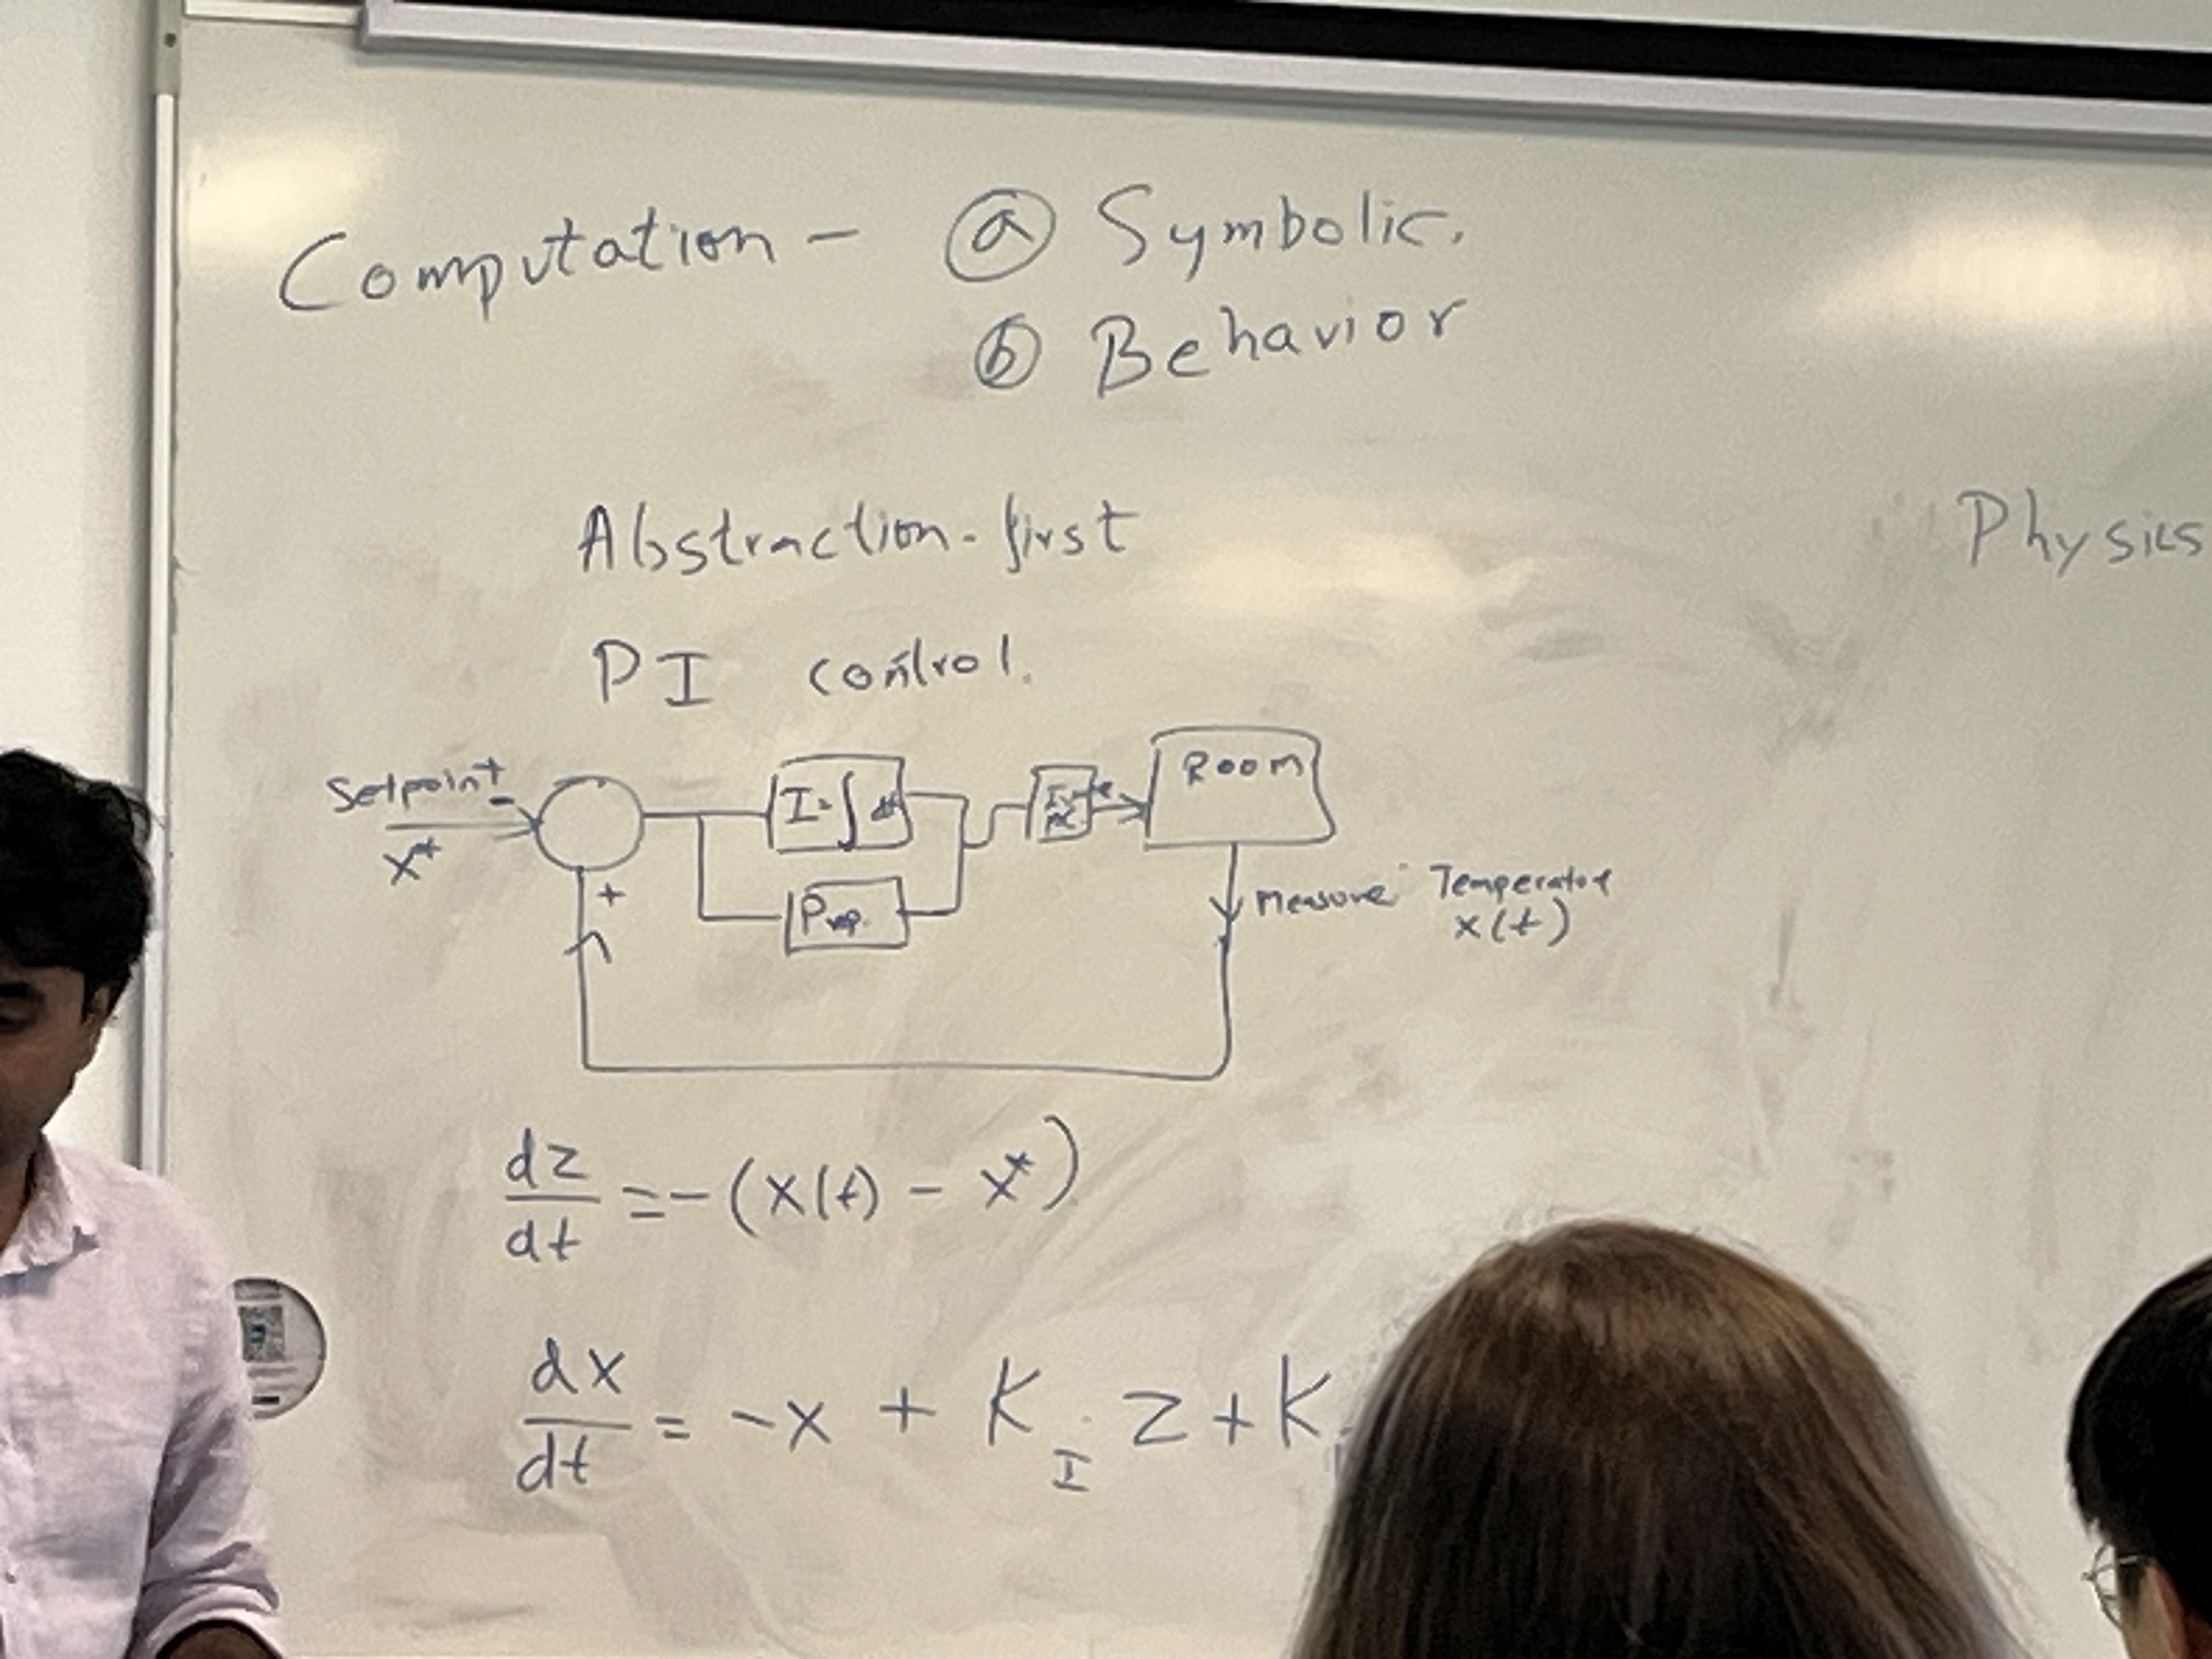
\includegraphics[scale=0.07]{figures/murugan/PI_Control.jpg}
		\caption{Diagram of control line}
	\end{figure*}\\
	This defines a differentiation equation which defines your control line $z$ due to observation of a process $x$
	\begin{itemize}
		\item Pros:
			\item General / modular
		\item Cons
			\item Cannot exploit specific physics
			\item The translation between theory vs implementation is non-trivial.
	\end{itemize}
	
	\item Physics First: 
	
	You can set up a thermodynamic state equation, and solve for the phase diagram.
	Pros and Cons
	\begin{itemize}
		\item Pros: 
			\item Fewer parts (measurement, computation), which means its more robust
			\item It's passive, meaning it self computes
		\item Cons
			\item Specific to the physics
	\end{itemize}
\end{enumerate}
This talk will focus on how to move toward the 2nd way of thinking. An example of this is the Liquid-Liquid phase transition of two liquids inside of a cell (see Zechnor 2020). You can think of this as oil and water separating.
\\
\\
There are two communities working on this
\begin{enumerate}
	\item Energy efficient computations (vs silicon). 
	\begin{itemize}
		\item Example. We currently run computations on a silicon chip, however this is not energy efficient, so much so governments are thinking about building more nuclear reactors to power the next generation of AI). So perhaps we can build biological circuits which run these computations natively on some bio-efficient chip.
		\item Example. Encode your optimization problem onto a Ising-like physical system, and anneal that system! Now you can read off optimized parameters.
		\item Example. You can use optimal computing to make better matrix multiplication.
	\end{itemize}
	\item Biological computations
	\begin{itemize}
		\item Backprop. That is each organism is reacting and adjusting it's behavior. Much more complex than just physics or chemical behavior.
		\item Evolution. No one organism does the computation, but rather it's the ensemble of them which can perform computations.
		\item Physics / Chemistry. It's just a reaction based on laws of physics / chemistry.
	\end{itemize}
\end{enumerate}
Now, how does this all relate to machine learning. Let's consider a high dimensional classifier-- you could think of the decision boundary as phase boundaries. You can also go one step further and use the transition between phases as the classifier (see \url{https://www.jbc.org/article/S0021-9258(20)36794-6/pdf} for more details)! So your features correspond to temperature, pressure, etc., and your classification is the phase. 
\begin{figure*}[h!]
	\centering
	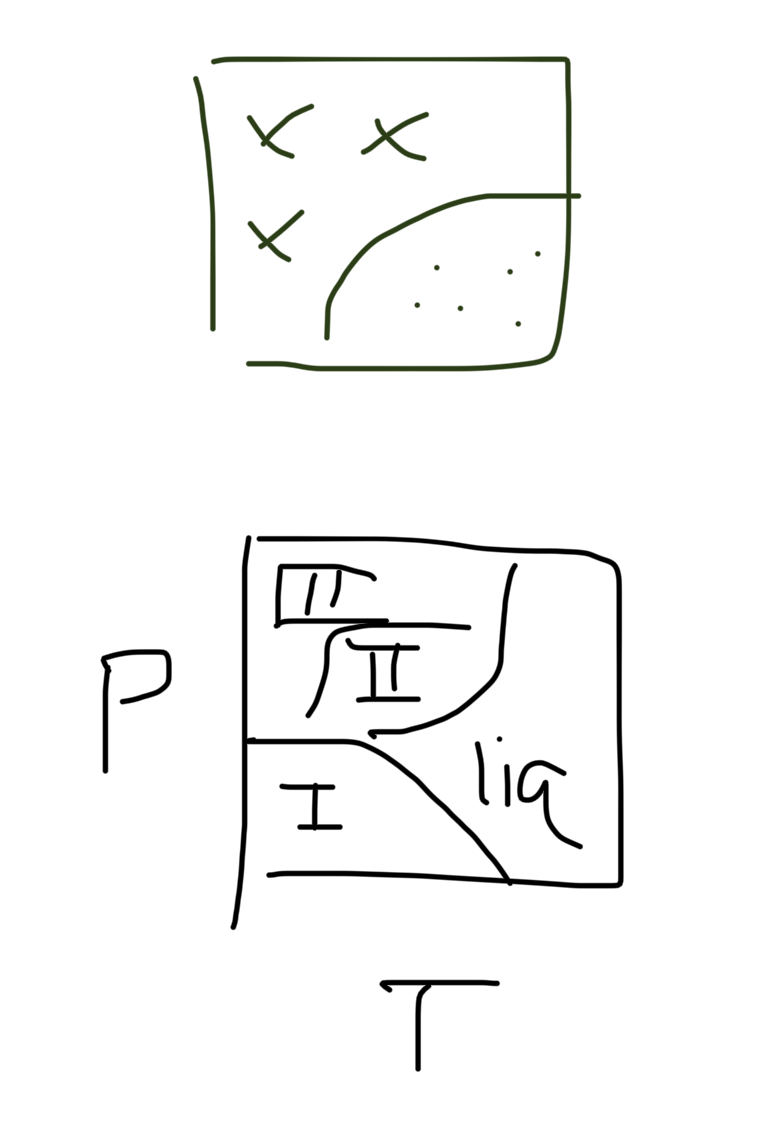
\includegraphics[scale=0.5]{figures/murugan/DecisionBoundary_PhaseDiagram.png}
	\caption{Decision boundary problems can be mapped into a physics system by inspecting their phase transition}
\end{figure*}
So the questions become what in the material / organism do I have to tune s.t. you can learn, and this also may find new interesting physical mechanisms for scientists to play with.

\subsection{Training Molecules}
\subsubsection{Hopefield Associative Memory}
Consider a set of neurons $\{x_i\}^N_{i=1}$ which take on binary values $x_i \in \{\pm 1\}$.  It takes on discrete dyanmics
\begin{align}
	x_i(t+1) = \text{sign}\left(\sum_j J_{ij} x_j(t) + h_i^{ext}(t) 
\right)
\end{align}
Your task is a supervised learning problem... The goal is to store a set of memories $m_i^\alpha \in \mathbb R^N$ (s.t. $\alpha = 1,..., M$). And you want to retrieve a memory $m$ from a just showing a partial part of $m$ (association). That is you want your neurons $\{x_i\}$ to fire in the same pattern as $m$ \\
\\
To train this model, we use a \textbf{Hebbian} learning rule
\begin{align}
	\frac{dJ_{ij}}{dt} = x_i (t) x_j(t)
\end{align}
We run this every time we should it a new memory. So for example, after being exposed to 3 memories $\{m^{(1)}, m^{(2)}, m^{(3)}\}$, our couplings look like $J_{ij} = m_i^{(1)} m_j^{(1)} + m_i^{(2)} m_j^{(2)} + m_i^{(3)} m_j^{(3)}$. Running this process will make the energy landscape become low where $x = m^{(i)}$-- so if you train on images, and then show noised versions of those images, then you'll be-able to denoise said images! Very cool! 

Note that hopfield networks have a memory capacity $M_c$, so this only works when the total memories $M < M_c$.

\subsubsection{Multifavious Assembly Mixtures}
Here we'll consider a physical system which is analogous to Hopfield's Assocative Memory model.

Consider $N$ molecular species in a solvent (this is different from the number of molecules, for example these can be $N$ proteins with different names), with binding interactions $J_{ij}$, and concentrations $C_i(x,t)$ at position $x$ at time $t$ (and associated chemical potentials $\mu_i$). The molecules are held at a physical temperature $T$, and have diffusion constant $D_i$.

\begin{align}
	\frac{dJ_{ij}}{dt} = - \int d^3x ~dt ~ C_i(x,t) C_j(x,t)
\end{align}
This rule says, these molecules will increase their bond ($J_{ij}$ will increase) if there are more of said molecules in the same place ($C_i(x,t) C_j(x,t)$ is the concentrations of molecules $i$ and $j$ at position $x$ at time $t$).

In practice, we need to use \textbf{linkers} (these are other molecules which mediate interactions between molecules). So they can be used to tune your $J_{ij}$'s.

The associative memory is to reconstruct a set of protein binded together. So you can construct a memory as a sequence of proteins, cut it up, place it into the test tube, and see if it can reconstruct the previous protein.


















\newpage


\newpage

\part{Etc.}

\section{People Presentations} 
\begin{enumerate}
	\item Paolo Balioni, working on feature learning in Bayesian Neural Networks. Also works on MCMC methods.
	\item Claudian Merger. Mappping normalizing flows to $\phi^n$ theory.
\end{enumerate}

\section{Acknowledgements}
Thank you to Prof. David Hogg \& the Flatiron Institute for providing funding for this trip!





\end{document}